\chapter{Field Test}

In order to test the rover's ability to localize itself, a simple field test was conducted in a parking lot. Inspiration for this experiment comes from Moore and Stouch \cite{robot_localization_paper}.
% An attempt was made to replicate the results in paper

\section{Experiment Design}

The rover was initially placed in a parking lot oriented westwards. It was then driven in a loop around the lot using the virtual\_joystick node, described in section \ref{sectionJoystick}. See Figure \ref{fig:roverPath} for two representations of the path taken. Figure \ref{figRouteMemory} displays the path actually traversed, while Figure \ref{figRouteGPS} is constructed from the phone's GPS readings. Note that despite Figure \ref{figRouteGPS}, at no point did the rover go onto the grass. The rover was driven so that its initial and ending position and orientation were roughly equal. Total collection time was five and a half minutes.

While the rover moved, raw sensor data streaming in from the Arduino and smartphone was recorded and saved into a ROS bag file.  Later, the \textit{rosbag} utility was used to repeatedly simulate the recorded sensor messages, while the EKF was run in different configurations. Refer to Table \ref{tab:configs} for a review of which state variables each sensor affects.

\section{Results}

% laptop had no problem computing using the filter. No memory spikes either. Very computationally efficient! laptop is enough for localization - is it enough for navigation?

During each filter computation, a state estimate was produced at 30 Hz in a local frame, and that output was then transformed into the global UTM frame, where position is given as latitude and longitude. These gps coordinates were plotted using the handy GPS Visualizer tool \cite{gps_visualizer} to generate the plots in  Figure \ref{fig:ekfOutputs}.

Figure \ref{figRouteOdom} shows the estimated path when feeding the filter only the wheel encoder odometry. The initial trajectory is off, but follows a straight path as expected. The first turn is tracked reasonably well, but the second turn rotates too far, so the final estimate never gets back to the starting position. It seems the wheel odometry estimate correctly measured the distance traveled, but had issues tracking yaw. Figure \ref{figRouteImu} shows the path generated when feeding the filter IMU data. While the scale is wildly off, the path has a good shape. It seems the IMU estimate greatly overestimated the distance traveled, but correctly measured the change in yaw caused by turning.

Figure \ref{figRouteOdomImuTwoYaw} shows the path generated when both wheel odometry and IMU data are fused into the filter. The path is now closer to truth in scale, but the shape could be better. Given our observation of the effects of both sensors individually, it seems reasonable to try to improve this output by ignoring the yaw tracking of the wheel encoders. This corresponds to changing \(\Psi'\) in Table \ref{tab:configs} from a 1 to a 0. Figure \ref{figRouteOdomImuOneYaw} shows the filter's output under this new configuration. The initial northern trajectory is still incorrect, but the rest of the path looks much better. If the initial heading were only fixed, it looks like this could be a good estimate of the true path.

% were impacted negatively during the field test by external magnetic fields other than the earth's. The field test itself was carried out in a parking lot filled with cars, some of which were running. Large metal bodies with flowing current cause large magnetic fields. 

Figure \ref{figRouteOdomImuGpsTwoYaw} shows the result of fusing both prior sensors with GPS fixes. This plot looks much like the raw gps plot in Figure \ref{figRouteGPS}, however upon closer inspection we can see jagged jumps in position. These jumps are instantaneous and actually lead to a discontinuous position estimate, though the visualizing tool connects every point. They are caused by the filter instantaneously adjusting the position estimate based on incoming gps fixes. The filter gives some weight to the current estimate, so the new adjusted position lies in between the position reported by the gps fix and the current estimate. Due to the frequent gps fixes and slow velocity of the rover, the estimated path never varies too far from the raw gps path. Figure \ref{figRouteOdomImuGpsOneYaw} again tries to improve the estimate by ignoring the yaw tracking of the wheel odometry. The output is fairly similar, but smoother.

\begin{table}[h]
	\caption {Errors for Different Sensor Fusions \cite{robot_localization_paper}} \label{tab:errors} 
	\begin{center}
		\begin{tabular}{|c|c|c|} \hline
			\textbf{Sensors Fused} & \textbf{Loop Closure Error x,y (m)} & \textbf{Std. Dev. x,y (m)} \\ \hline
			Wheel Encoders & -88.53, -55.51 & 61.81, 130.76 \\ \hline
			IMU & 
			1247.12, -355.66 &
			1786.48, 3351.81 \\ \hline
			Encoders(Yaw) + IMU &
			-16.71, -14.57 &
			50.71, 57.88  \\
			\hline
			Encoders(No Yaw) + IMU &
			7.40, 2.53 &
			65.64, 40.15  \\
			\hline
			Encoders(Yaw) + IMU + GPS & 0.51, -1.06 & 4.55, 4.67 \\ \hline
			Encoders(No Yaw) + IMU + GPS & 0.49, -1.06 & 4.55, 4.67 \\ \hline
		\end{tabular}
	\end{center}
\end{table}

Table \ref{tab:errors} shows the position error between the rover's start and end positions for each filter configuration. Because the rover's local frame has its origin at the start point, this error is simply the last state estimate produced by the filter. The standard deviation for each dimension is also reported, giving an idea of the filter's confidence in its location. The estimates when gps is not used are gathered from the continuous odom frame, and their error grows without bound. The estimates from when gps was fused are gathered from the discrete map frame, and its error is bounded by the variance of the gps fix. Note that because the rover initially started facing north-west, negative x or y closure errors refer to either south-east or north-east, respectively.

\begin{figure}[p] 
	\caption{
		The Rover's Path
	}
	\label{fig:roverPath}
	\begin{subfigure}{\textwidth}
		\centering
		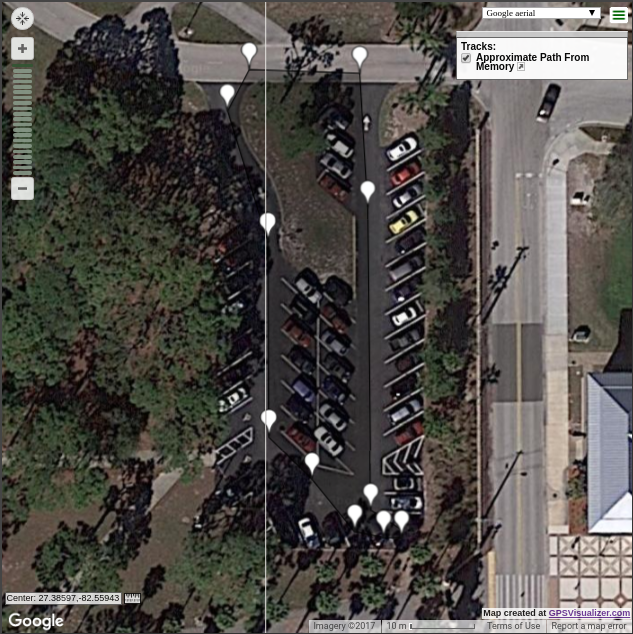
\includegraphics[height=0.45\textheight]{testRun/route_from_memory}
		\caption{Path Manually Mapped}
		\label{figRouteMemory}
	\end{subfigure}
	\begin{subfigure}{\textwidth}
		\centering
		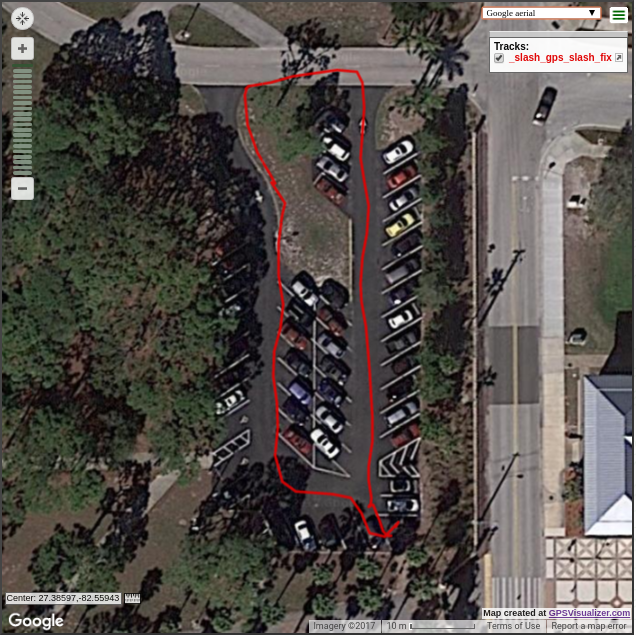
\includegraphics[height=0.4\textheight]{testRun/raw_gps_data}
		\caption{Path According to Phone's GPS}
		\label{figRouteGPS}
	\end{subfigure}
	
\end{figure}

\begin{figure}[p] 
	\caption{
		Filter Outputs For Different Sensor Fusions
	}
	\label{fig:ekfOutputs}
	\begin{subfigure}{\textwidth}
		\centering
		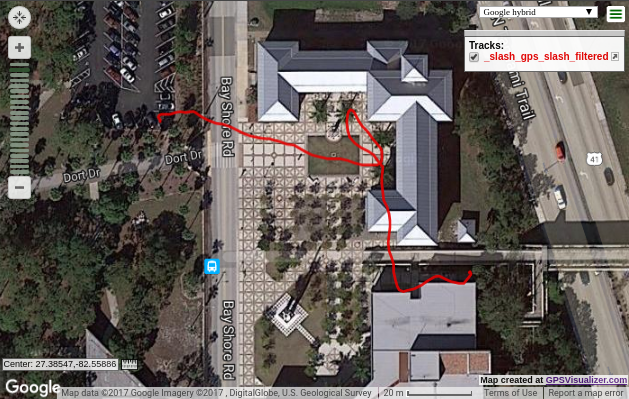
\includegraphics[height=0.4\textheight]{testRun/ekf_output_odom}
		\caption{Raw Wheel Odometry}
		\label{figRouteOdom}
	\end{subfigure}
	\begin{subfigure}{\textwidth}
		\centering
		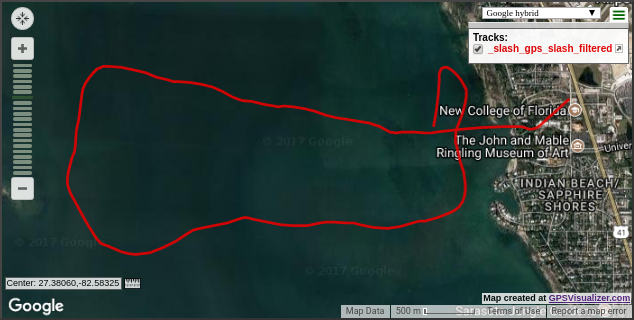
\includegraphics[height=0.4\textheight]{testRun/ekf_output_imu}
		\caption{IMU}
		\label{figRouteImu}
	\end{subfigure}
\end{figure}

\begin{figure}[p] \ContinuedFloat
\begin{subfigure}{\textwidth}
	\centering
	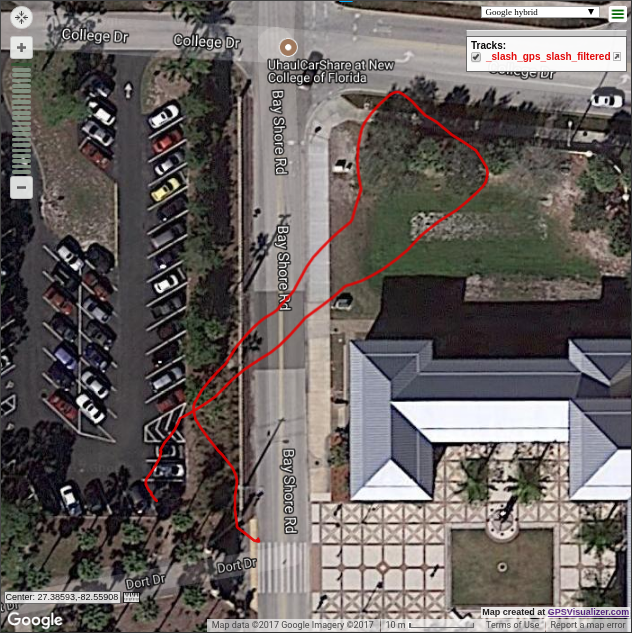
\includegraphics[height=0.4\textheight]{testRun/ekf_output_odom_imu_two_yaw}
	\caption{Wheel Odometry + IMU (Wheel Odometry affects yaw)}
	\label{figRouteOdomImuTwoYaw}
\end{subfigure}
\begin{subfigure}{\textwidth}
	\centering
	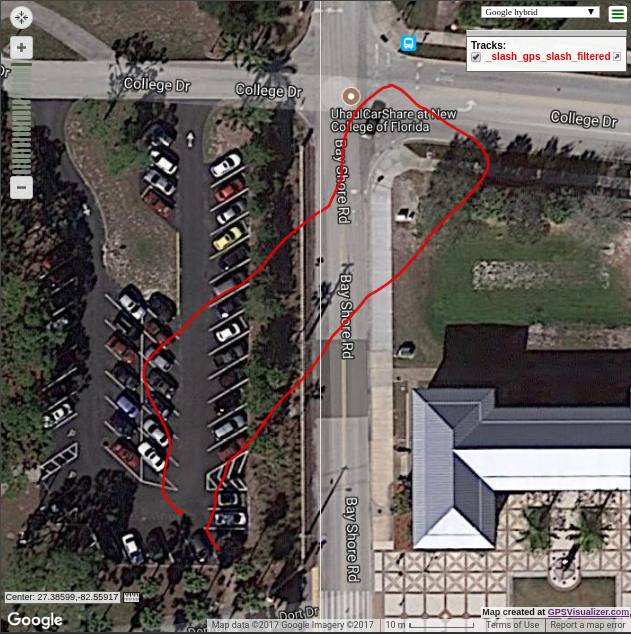
\includegraphics[height=0.4\textheight]{testRun/ekf_output_odom_imu_one_yaw}
	\caption{Wheel Odometry + IMU (Wheel Odometry does not affect yaw)}
	\label{figRouteOdomImuOneYaw}
\end{subfigure}
	
\end{figure}

\begin{figure}[p] \ContinuedFloat
	\begin{subfigure}{\textwidth}
		\centering
		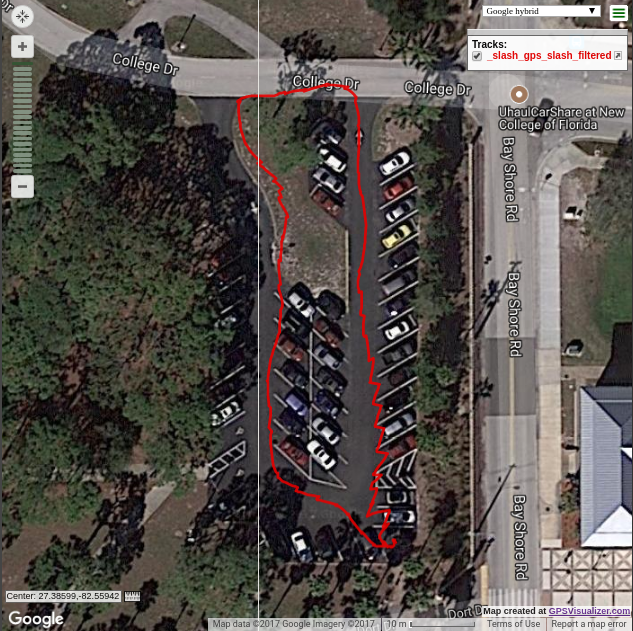
\includegraphics[height=0.4\textheight]{testRun/ekf_output_odom_imu_gps_two_yaw}
		\caption{Wheel Odometry + IMU + GPS (Wheel Odometry affects yaw)}
		\label{figRouteOdomImuGpsTwoYaw}
	\end{subfigure}
	\begin{subfigure}{\textwidth}
		\centering
		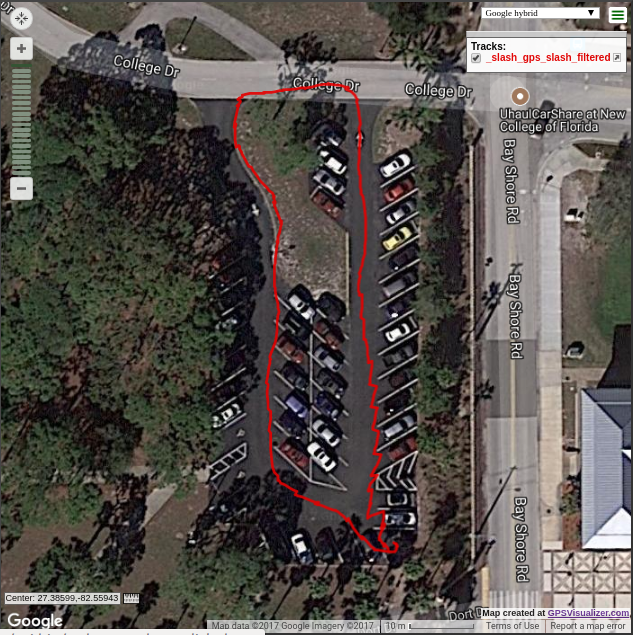
\includegraphics[height=0.4\textheight]{testRun/ekf_output_odom_imu_gps_one_yaw}
		\caption{Wheel Odometry + IMU + GPS (Wheel Odometry does not affect yaw)}
		\label{figRouteOdomImuGpsOneYaw}
	\end{subfigure}
\end{figure}